\documentclass[11pt]{article}
\usepackage[margin=1.1in]{geometry}
\usepackage[T1]{fontenc}
\usepackage{lmodern}
\usepackage{microtype}
\usepackage{natbib}
\usepackage{float}
\usepackage{tikz}
\usetikzlibrary{arrows.meta,positioning,calc,fit}
\usepackage{../shared/smcbvs}
\bibliographystyle{abbrvnat}
\setcitestyle{authoryear,round}
\linespread{1.08}
% code locations: paths relative to Scripts/SMC_BVS/core/
\usepackage{url}
\makeatletter\g@addto@macro\UrlBreaks{\do\_\do\-\do\:}\makeatother
\urlstyle{tt}
\DeclareUrlCommand\code{}
\setlength{\emergencystretch}{3em}
\newcommand{\Nc}{N^{\mathrm c}}   % calibration particles
\newcommand{\grid}[1]{\phi_{[#1]}}  % temperatures of the grid
\newcommand{\grouprow}[1]{\midrule\multicolumn{6}{@{}l}{\textbf{#1}}\\}

\title{The SMC-BVS method, as coded}
\author{SMC-BVS project}
\date{Draft, \today}

\begin{document}
\maketitle

\begin{abstract}
\noindent
This part of the paper describes the SMC-BVS method exactly as the software implements it: how it prepares the data, the
model and every prior, the posterior it targets, and each step of the algorithm, from the start law to the reported
outputs. The user supplies the data, a random seed and a computing allocation. In the default configuration, which is the
one described here, everything else is either a numerical constant or a stated function of the sample size $n$ and the
number of predictors $p$. A parameter table gives the constants with their locations in the code. The theorems of the companion
part are about this method.
\end{abstract}

% =====================================================================================================
\section{Setup and notation}\label{sec:m-setup}

This section introduces the notation of the paper, the data, and the way the method prepares them. The method sees the
data only after centring and scaling, and every later quantity is defined on that scale. The model that generates the
data, and the true parameter values, are introduced in the companion part.

\subsection{Notation}\label{sec:m-notation}

For an integer $k\ge1$ we write $\set{k}:=\{1,\dots,k\}$. Vectors are columns. The Euclidean norm of a vector $v$ is
$\norm{v}$ and its $\ell_1$ norm is $\norm{v}_1$. An identity matrix is written $I_n$, or $I$ when its size is clear,
and $\one_n$ (or $\one$) is the vector of ones. The smallest eigenvalue of a symmetric matrix is written $\lmin(\cdot)$.
The number of elements of a set $S$ is $\abs{S}$. Logarithms are natural ($\log$) or binary ($\log_2$);
$\lceil\cdot\rceil$ and $\lfloor\cdot\rfloor$ round up and down; $a\vee b:=\max(a,b)$; and $\ind{E}$ is the indicator of
an event or condition $E$. A star on a parameter marks its true value; the superscript $\mathrm r$ marks raw,
unstandardised data. For a $p\times p$ matrix $\Lambda$ and sets $U,V\subseteq\set{p}$, $\Lambda_{UV}$ is the sub-matrix
with rows in $U$ and columns in $V$, and $\Lambda_U:=\Lambda_{UU}$.

For random variables $V_n$ and positive numbers $a_n$, $V_n=\OP(a_n)$ means that for every $\epsilon>0$ there is a
constant $C$ with $\P(\abs{V_n}>Ca_n)\le\epsilon$ for all large $n$, and $V_n=\oP(a_n)$ means $V_n/a_n\to0$ in
probability; \emph{with probability tending to one} means that the probability of the event tends to one. For positive
sequences, $a_n=O(b_n)$ (also $a_n\lesssim b_n$) means $a_n\le Cb_n$ for a constant $C$; $a_n=o(b_n)$ means
$a_n/b_n\to0$; $a_n\asymp b_n$ means $a_n\lesssim b_n$ and $b_n\lesssim a_n$; $a_n\gg b_n$ means $b_n/a_n\to0$; and
$a_n\gtrsim b_n$ means $b_n\lesssim a_n$. A quantity is \emph{fixed} if it does not depend on $n$. Some of this notation is
used only in the companion part.

\subsection{The data}\label{sec:m-data}

\paragraph{Inputs.} A \emph{run} is one call of the software. It receives a response vector $\yr\in\R^n$, an $n\times\praw$
matrix of predictors, a random \emph{seed} and a computing \emph{allocation} (memory and time; by default 8\,GiB, that is $8\cdot2^{30}$ bytes, and 24
hours). The inputs are \emph{valid} when $n\ge3$, at least one predictor is given and every entry is a finite number; the
seed is valid when it is an integer in $\{1,\dots,2^{31}-1\}$. Invalid inputs stop the run.

\paragraph{Removing constant predictors.} A predictor whose entries are all exactly equal is removed, and the method
records which predictors were removed. A constant predictor is a multiple of $\one_n$, so its effect is absorbed by the
intercept. We write $\Xr$ for the $n\times p$ matrix of the $p$ \emph{retained} predictors (still raw, that is,
unstandardised), indexed by $\set{p}$. From here
on, $p$ always means this number: the prior, the size cap and every score use the retained predictors only. If no
predictor is retained, or if the response is constant, the method stops and reports the empty model.

\paragraph{Standardisation.} The method centres and scales every retained predictor and the response. Let
$P^\perp_{\one}:=I_n-n^{-1}\one\one^\top$ be the centring matrix and $D$ the $p\times p$ diagonal matrix of the sample
standard deviations (divisor $n-1$) of the columns of $\Xr$. The method works with
\begin{equation}\label{eq:m-standardise}
  X:=P^\perp_{\one}\Xr D^{-1},\qquad y:=P^\perp_{\one}\yr/s_y,\qquad s_y^2:=\norm{P^\perp_{\one}\yr}^2/(n-1).
\end{equation}
So every column $x_j$ of $X$ has mean zero and $\norm{x_j}^2=n-1$, and $y$ has mean zero and $y^\top y=n-1$. (In
floating point, each column is first divided by its largest absolute value, which leaves~\eqref{eq:m-standardise}
unchanged; a numerically stable two-pass centring is used when a column is nearly constant.)

\paragraph{Models.} A \emph{model} is a set $S\subseteq\set{p}$ of predictors. For a model $S$: $X_S$ is the matrix of
the columns of $X$ in $S$; $G_S:=X_S^\top X_S$ is their Gram matrix; $\Rhat_S:=G_S/(n-1)$ is their sample correlation
matrix; $\hat r_{jl}$ is the sample correlation of predictors $j$ and $l$; $P_S$ is the orthogonal projection onto the span of the columns of $X_S$
($P_\emptyset:=0$); and $z_S:=X_S^\top y$.

\paragraph{The intercept.} The intercept is not a parameter of the working model: it is removed by centring $X$ and $y$.

\paragraph{Duplicated predictors.} Two predictors whose sample correlation is at least $1-10^{-10}$ in absolute value are
reported as duplicates. Both are kept.

% =====================================================================================================
\section{The model and the prior}\label{sec:m-prior}

The method fits a Gaussian linear model to the standardised data and puts a prior on its three unknowns: which
predictors are in the model, their coefficients, and the noise variance. Every hyperparameter is a numerical constant
or a function of $(n,p)$; the prior rows of Table~\ref{tab:m-params} give each one with its code location.

\paragraph{Working model.} Given a model $S$, coefficients $\theta_S\in\R^{\abs{S}}$ and a variance $\sigma^2>0$,
\begin{equation}\label{eq:m-working}
  y\mid S,\theta_S,\sigma^2\ \sim\ \Normal_n(X_S\theta_S,\sigma^2I_n).
\end{equation}
In words: the standardised response is a linear function of the predictors in $S$ plus independent Gaussian noise. Here
$\theta_S$ and $\sigma^2$ are working parameters, not true values. The theorems are proved under the data-generating
model of the companion part, not under this working model.

\paragraph{Model space and size cap.} The method considers every model with at most $K$ predictors:
\begin{equation}\label{eq:m-space}
  \Om:=\{S\subseteq\set{p}:\abs{S}\le K\},\qquad K:=\min\big(p,\lfloor n/2\rfloor\big).
\end{equation}
The cap is a function of $(n,p)$: models with more than $n/2$ predictors are never scored.

\paragraph{Model prior.} The prior probability of a model depends only on its size $k=\abs{S}$:
\begin{equation}\label{eq:m-modelprior}
  \text{prior probability of }S=\frac{w(\abs{S})}{\bar w_K},\qquad w(k):=\frac{1}{2\binom{2p-1}{k}},\qquad
  \bar w_K:=\sum_{k=0}^{K}\binom{p}{k}w(k).
\end{equation}
This is the beta-binomial prior $\BB(1,p)$ \citep{ScottBerger2010}, restricted to $\Om$. A probability $q$ is drawn from
$\BetaDist(1,p)$, and, given $q$, each predictor enters the model independently with probability $q$; then a given model
of size $k$ has probability $\mathcal B(k+1,2p-k)/\mathcal B(1,p)=w(k)$, where $\mathcal B$ is the beta function. Dividing by
$\bar w_K$ renormalises the prior to models of size at most $K$. The second parameter of the beta distribution is $p$, the
number of retained predictors, so the prior is a function of $p$ and its cap a function of $(n,p)$. The prior mean model
size is about one. Adding one predictor to a model of size $k$ multiplies the prior weight by $(k+1)/(2p-1-k)$: one more
predictor costs about $\log\{2p/(k+1)\}$ in log prior odds, so the prior penalises size more when $p$ is large.

\begin{example}[The model prior with three predictors]\label{ex:m-prior}
Take $p=3$ and $n\ge6$, so that $K=3$ and no model is excluded. Then $w(0)=\tfrac12$, $w(1)=\tfrac1{10}$ and
$w(2)=w(3)=\tfrac1{20}$, and $\bar w_K=\tfrac12+3\cdot\tfrac1{10}+3\cdot\tfrac1{20}+\tfrac1{20}=1$. So the empty model has
prior probability $\tfrac12$; each one-predictor model $\tfrac1{10}$ (together $\tfrac3{10}$); each two-predictor model
$\tfrac1{20}$ (together $\tfrac3{20}$); and the full model $\tfrac1{20}$. Small models are favoured, and each extra
predictor must earn its place through the data. With $n=4$ instead, $K=2$, the full model is excluded, and
$\bar w_K=\tfrac{19}{20}$: the remaining seven models are renormalised.
\end{example}

\paragraph{Coefficients.} Given $S$ and $\sigma^2$, the coefficients have the ridge-stabilised $g$-prior
\citep{Zellner1986} with $g=n$:
\begin{equation}\label{eq:m-slab}
  \theta_S\mid S,\sigma^2\ \sim\ \Normal\big(0,\;n\sigma^2(G_S+I)^{-1}\big).
\end{equation}
In words: the prior covariance is $n\sigma^2$ times the inverse of the Gram matrix with a unit ridge added. The factor
$g=n$ makes the prior worth about one observation; the ridge $I$ keeps the prior proper when $G_S$ is singular. The method
never forms this prior explicitly: \eqref{eq:m-slab} is the Gaussian prior whose marginal likelihood is the
formula~\eqref{eq:m-marglik} that the method evaluates.

\paragraph{Noise variance.} $\sigma^2\sim\IG(a_0,b_0)$, inverse gamma with shape $a_0=0.01$ and scale $b_0=0.01$: a weak,
proper prior.

% =====================================================================================================
\section{The posterior}\label{sec:m-posterior}

Because the prior is conjugate, the coefficients and the noise variance integrate out in closed form, and the posterior
over models is known up to one constant. The method's target is exactly this posterior.

\paragraph{Marginal likelihood.} Integrating $\theta_S$ and $\sigma^2$ out of~\eqref{eq:m-working}--\eqref{eq:m-slab}
gives
\begin{equation}\label{eq:m-marglik}
  m(S)=C_n\Big(\frac{\det H_S}{\det(G_S+I)}\Big)^{-1/2}(2b_0+\SSq_S)^{-\nu},
\end{equation}
where $H_S:=(n+1)G_S+I$ and $\SSq_S:=y^\top y-n\,z_S^\top H_S^{-1}z_S$,
with $\nu:=a_0+n/2$ and $C_n:=(2b_0)^{a_0}\Gamma(a_0+n/2)/\{\pi^{n/2}\Gamma(a_0)\}$ (here $\pi$ is the number $3.14\ldots$).
For the empty model, $m(\emptyset)=C_n(2b_0+y^\top y)^{-\nu}$. In words: $\SSq_S$ is a shrunken residual sum of squares,
so models that fit better have larger $m(S)$. The determinant ratio is a penalty for model size (an Occam factor). In a
well-conditioned model it alone multiplies $m(S)$ by about $(n+1)^{-1/2}$ for each extra predictor, and a better fit,
through $\SSq_S$, can more than make up for it.

\paragraph{How the score is computed.} The method tries three computations in turn: a Cholesky factorisation of $H_S$;
the same after recomputing the Gram matrix from $X$; and a QR factorisation. It reports a numerical failure only if all
three fail. When $\SSq_S$ is very small (below $10^{-8}\,y^\top y$), it is recomputed in the non-negative form
$\norm{y-X_Sb}^2+(\norm{X_Sb}^2+\norm{b}^2)/n$ with $b:=nH_S^{-1}z_S$. To \emph{score} a model is to compute $\log m(S)$,
and hence $F(S)$ below; a \emph{score request} asks for one such computation, possibly answered from a cache.

\paragraph{Log score and posterior.} The \emph{log score} of a model is
\begin{equation}\label{eq:m-score}
  F(S):=\log\{w(\abs{S})/\bar w_K\}+\log m(S),
\end{equation}
the logarithm of its prior probability times its marginal likelihood. The \emph{posterior over models} is
\begin{equation}\label{eq:m-posterior}
  \pis{S}=\frac{e^{F(S)}}{Z},\qquad Z:=\sum_{S'\in\Om}e^{F(S')},\qquad S\in\Om .
\end{equation}
The normalising constant $Z$ is the \emph{evidence}: the marginal likelihood of the standardised data under the working
model and the prior. Because $y$ is standardised, the posterior over models does not change if $\yr$ is shifted or
rescaled.

\paragraph{Posterior summaries.} The \emph{posterior inclusion probability} of predictor $j$ is
$\PIP_j:=\sum_{S\ni j}\pis{S}$; the \emph{highest posterior model} is $\HPM:=\argmax_{S\in\Om}\pis{S}$; and the
\emph{median probability model} is $\MPM:=\{j:\PIP_j>1/2\}$ \citep{BarbieriBerger2004}. The method estimates these, and
$Z$.

% =====================================================================================================
\section{Why sequential Monte Carlo, and why this start law}\label{sec:m-intuition}

This section explains, without formulas, why the method has the stages it has. The next section gives each stage in
detail.

The posterior is known up to one constant, so the difficulty is not computing it but finding where its mass is: the
model space is enormous and rugged. It is rugged for two reasons. Correlated predictors create near-ties between models
that differ by swapping a true predictor for its proxy. And a predictor that is useless once the true ones are in can look
useful on its own: it \emph{leaks} part of their signal.

A Markov chain started at an arbitrary model can spend a long time stuck near one of these near-ties. Sequential Monte
Carlo avoids that by starting from a distribution that is easy and already close to the target, and by moving towards the
target in small steps, with many models (\emph{particles}) at once. At each step the particles that the next distribution
favours are copied and the others dropped, and Markov moves spread the copies out again. The independence moves, drawn
from the start law, let particles jump between near-equivalent models in one step. Four independent copies of the sampler
(\emph{islands}) give a check of stability.

The \emph{start law}, an exactly computable approximation of the posterior, is that easy, close distribution. It resolves exactly the hardest local competition, a true predictor
against its close proxies, because correlated predictors tend to land in the same block, where every subset is scored.
It can be normalised and sampled exactly, so the particles start from independent draws, and the evidence estimate starts
from the exactly known normaliser of the start law. What it gets wrong is leakage across blocks. The local search from the start mode undoes that: it deletes
the spurious predictors one per move. Because this search uses no random numbers, it gives a second, deterministic route
to the true model that does not depend on how well the particles mixed.

Finally, the calibration fits the sequence of distributions to the data set and then freezes it before the final run.
Because the schedule is fixed before the final run draws any random number, the final run is a standard sequential
Monte Carlo sampler with a fixed schedule; the companion part's results on the reported estimates assume exactly this.

% =====================================================================================================
\section{The algorithm, step by step}\label{sec:m-algorithm}

A run has seven stages (Figure~\ref{fig:m-pipeline}). Small problems are solved exactly. Otherwise the method builds the
start law, an exactly computable approximation of the posterior; calibrates a sequence of distributions from the start
law to the posterior; moves four independent sets of particles along that sequence; and finishes with two deterministic
local searches. The models it scores are recorded, and the one with the highest log score is reported
(Section~\ref{sec:m-outputs}). We describe one island (Section~\ref{sec:m-island}) before the calibration
(Section~\ref{sec:m-calibration}), because the calibration is built from islands. In this section a \emph{stage} is one
of the seven boxes of Figure~\ref{fig:m-pipeline}; a \emph{step} is one move of the sampler from one temperature to the
next.

\begin{figure}[ht]
\centering
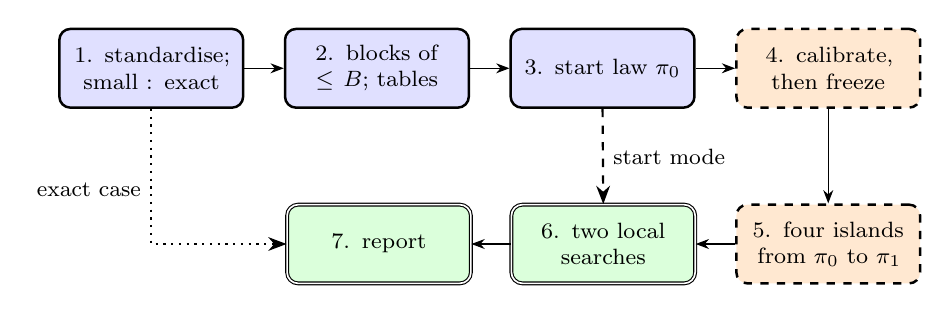
\begin{tikzpicture}[node distance=5mm, every node/.style={font=\footnotesize},
  box/.style={draw, rounded corners, align=center, minimum height=10mm, text width=21mm},
  exact/.style={box, fill=blue!12, line width=0.9pt}, stoch/.style={box, fill=orange!18, dashed, line width=0.9pt},
  det/.style={box, fill=green!14, double}]
\node[exact] (pre) {1. standardise;\\ small $\Om$: exact};
\node[exact, right=of pre] (blk) {2. blocks of\\ $\le B$; tables};
\node[exact, right=of blk] (start) {3. start law $\pi_0$};
\node[stoch, right=of start] (cal) {4. calibrate,\\ then freeze};
\node[stoch, below=12mm of cal] (smc) {5. four islands\\ from $\pi_0$ to $\pi_1$};
\node[det, left=of smc] (ls) {6. two local\\ searches};
\node[det, left=of ls] (out) {7. report};
\draw[-{Stealth}] (pre)--(blk); \draw[-{Stealth}] (blk)--(start); \draw[-{Stealth}] (start)--(cal);
\draw[-{Stealth}] (cal)--(smc); \draw[-{Stealth}] (smc)--(ls); \draw[-{Stealth}] (ls)--(out);
\draw[-{Stealth}, dashed, thick] (start.south) -- node[right, pos=0.5]{start mode $\tSz$} (ls.north);
\draw[-{Stealth}, dotted, thick] (pre.south) |- node[left, pos=0.3]{exact case} (out.west);
\end{tikzpicture}
\caption{The stages of a run. Exact computations: solid boxes (1--3). Random: dashed boxes (4--5). Deterministic given
their inputs: double boxes (6--7). When $\Om$ is small the run goes from stage~1 straight to the report (dotted). The
second local search starts from the start mode and does not depend on the particles (dashed arrow).}
\label{fig:m-pipeline}
\end{figure}

\subsection{The exact case, the check before the run, and the effort tiers (stage 1)}\label{sec:m-budgets}

\paragraph{The exact case.} The method first decides whether to enumerate. Let $N_0:=\max(2500,n,p)$ and
$\Nc_0:=\lceil512N_0/2500\rceil$ (the particle numbers of Sections~\ref{sec:m-island} and~\ref{sec:m-calibration}). If
$\abs{\Om}=\sum_{k\le K}\binom pk$ is at most $(5\Nc_0+4N_0)\,p$, the method scores every model and computes $Z$, every
inclusion probability, the highest posterior model and the median probability model exactly (Section~\ref{sec:m-outputs}
lists what it reports). No random number is used. Otherwise it proceeds to stage~2.

\paragraph{The check before the run.} After the data preparation of Section~\ref{sec:m-data} and before stage~2, the
method estimates what the run will need, and stops with status ``resource limit'' if the estimate exceeds the
allocation. In the exact case it estimates the memory and the time of the
enumeration (from 200 timed scores). For the sampler it estimates the memory, and, in the default configuration, also the
worst-case time of the local search from the start mode (stage~6): with $\ell_n:=\lceil\log_2(n+p+1)\rceil$, at most
$\ell_n+K+1$ full scans of at most $p+p^2/4$ models each, so $(\ell_n+K+1)(p+p^2/4)$ score requests, each costed at twice
the measured time to score one model of size $K$. At $n=200$ and $p=10^4$ that is about $2.9\times10^9$ requests, so the default 24-hour allocation passes
only if one score of a 100-predictor model takes less than about $1.5\times10^{-5}$ seconds; larger problems need a larger
time allocation. The same check is repeated before the calibration moves to tier~1 (the memory estimate grows with the
number of particles).

\paragraph{Effort tiers.} The sampler has two effort tiers, $i\in\{0,1\}$. Tier $1$ multiplies the number of particles and
the step ceiling $T_i$ (Section~\ref{sec:m-calibration}) of tier $0$ by four. The calibration starts at tier $0$ and moves to tier $1$ at most once
(Section~\ref{sec:m-calibration}). All effort constants are functions of $(n,p)$ alone; Table~\ref{tab:m-params} lists
them.

\subsection{Blocks and block tables (stage 2)}\label{sec:m-blocks}

The method partitions the predictors into blocks $C_1,\dots,C_J$ of at most $B:=\min(\lfloor\sqrt n\rfloor,\lfloor\sqrt
p\rfloor,16)$ predictors each. It clusters the predictors by complete-linkage hierarchical clustering on the dissimilarity
$1-\abs{\hat r_{jl}}$, with fixed tie-breaking rules. It then cuts the tree top-down: starting from the root, every
cluster with more than $B$ members is replaced by its two sub-clusters, until every cluster has at most $B$ members.
Finally it packs whole clusters into blocks in the order of the tree's leaves, starting a new block whenever the next
cluster does not fit (next-fit packing), and sorts each block. The partition is therefore a deterministic function of
$X$, and correlated predictors tend to share a block.

Within each block $C_b$ the method scores every subset $U\subseteq C_b$ with $\abs{U}\le K$ against the full response,
and stores the \emph{block table} $r_b(U):=m(U)/m(\emptyset)$, with $r_b(\emptyset)=1$. A block has at most $2^{16}$
subsets, so the tables are cheap.

The method also builds a \emph{neighbour graph}, used by the swap moves of Section~\ref{sec:m-island}. For each predictor
$j$ it keeps the predictors $l$ with $\abs{\hat r_{jl}}>\sqrt{2\log p/n}$, in decreasing order of $\abs{\hat r_{jl}}$, at
most $B$ of them; if none passes the threshold, it keeps the most correlated one. It then makes the graph symmetric by
union (it adds $j$ to the neighbours of $l$ whenever $l$ is a neighbour of $j$), so that every neighbour swap can be
reversed. We write $\mathcal N(j)$ for the set of $j$'s neighbours; after the union it may have more than $B$ members.

\subsection{The start law (stage 3) and the start mode}\label{sec:m-start}

\paragraph{The start law.} The start law multiplies the size prior by the block tables:
\begin{equation}\label{eq:m-startlaw}
  \pi_0(S)=\frac{\gamma_0(S)}{\bar Z_0},\qquad \gamma_0(S):=\frac{w(\abs{S})}{\bar w_K}\prod_{b=1}^J r_b(S\cap C_b),\qquad
  \bar Z_0:=\sum_{S\in\Om}\gamma_0(S).
\end{equation}
In words: $\pi_0$ is the posterior one would have if the marginal likelihood of a model, relative to the empty model, split
into independent contributions from the blocks. It sees every interaction within a block and none between blocks; the size prior still couples the blocks.

The normaliser $\bar Z_0$ is computed exactly by a recursion over model sizes. Let $E_b(k):=\sum_{U\subseteq C_b,\,\abs{U}=k}
r_b(U)$ be the total table weight of the subsets of block $b$ of size $k$ ($E_b(k)=0$ for $k>\min(\abs{C_b},K)$). Then
\[
  \Phi_0(k):=\ind{k=0},\qquad \Phi_b(k):=\sum_{k'=0}^{k}\Phi_{b-1}(k-k')\,E_b(k'),\qquad
  \bar Z_0=\sum_{k=0}^{K}\frac{w(k)}{\bar w_K}\,\Phi_J(k).
\]
Here $\Phi_b(k)$ is the total table weight of all ways to choose subsets in blocks $1,\dots,b$ with $k$ predictors in all.
The same recursion gives an exact sampler. Draw the total size $k$ with probability proportional to
$\{w(k)/\bar w_K\}\Phi_J(k)$. Then, backwards from $b=J$, with $k_J:=k$ predictors still to place in blocks $1,\dots,b$,
give block $b$ the size $k'$ with probability $\Phi_{b-1}(k_b-k')E_b(k')/\Phi_b(k_b)$, and set $k_{b-1}:=k_b-k'$. Finally,
in each block, draw a subset of the allotted size with probability proportional to $r_b(U)$, among the subsets of that
size. So $\pi_0$ can be computed and sampled exactly.

\paragraph{The start mode.} The \emph{start mode} $\tSz$ is a maximiser of $\pi_0$ over $\Om$ (the tilde distinguishes it
from the true model $\Sz$ of the companion part). It is computed at the end of the run, where the second local search
needs it (stage~6), by the same recursion with sums replaced by maxima. If maximisers of different sizes exist, the
method keeps those of the smallest size; among them it returns the lexicographically smallest set (comparing the
increasingly sorted index vectors). It lists the maximisers when there are fewer than $10^6$ of them, and otherwise uses a
version of the recursion that tracks ties and returns the same set without listing them.

\paragraph{The discrepancy.} The start law and the posterior differ by the \emph{discrepancy}
\begin{equation}\label{eq:m-discrepancy}
  d(S):=\log\frac{m(S)}{m(\emptyset)}-\sum_{b=1}^J\log r_b(S\cap C_b),
\end{equation}
the part of the log marginal likelihood of $S$ (relative to the empty model) that comes from interactions between
blocks. Then $\gamma_0(S)e^{d(S)}=e^{F(S)}/m(\emptyset)$,
which is proportional to the posterior.

\begin{example}[Leakage, with six predictors]\label{ex:m-toy}
Take $n=100$ and six predictors, with true model $\{1,3\}$, both coefficients $1$, and unit noise. Predictor $2$ is a
\emph{proxy} of $1$ (correlation $0.93$); $4$ is moderately correlated with $3$ ($0.69$); $5$ is correlated with $1$
($0.63$); and $6$ is a proxy of $5$ ($0.89$). Here $B=2$, and the blocks are $\{1,2\}$, $\{3,4\}$ and $\{5,6\}$: the proxy $2$
shares predictor $1$'s block, while predictor $5$ sits in a different block from the true predictor whose signal it
carries. The five models with the largest posterior mass are (the first three are also the three with the largest
start-law mass):

\smallskip
\centerline{\small
\begin{tabular}{@{}lccccc@{}}
\toprule
model & $\{1,3,5\}$ & $\{1,3\}$ & $\{1,3,6\}$ & $\{1,3,4\}$ & $\{1,2,3\}$ \\
\midrule
start law $\pi_0$ & $\mathbf{0.517}$ & $0.198$ & $0.067$ & $0.012$ & $0.008$ \\
posterior $\pi(\cdot\mid y)$ & $0.042$ & $\mathbf{0.688}$ & $0.118$ & $0.051$ & $0.037$ \\
\bottomrule
\end{tabular}}
\smallskip

Within its own block, predictor $5$ explains much of $y$, because it carries part of predictor $1$'s signal, and the start
law cannot see that predictor $1$, in another block, already explains it. So the start mode is $\{1,3,5\}$: predictor $5$
\emph{leaks}. The proxy $2$, in predictor $1$'s own block, is handled correctly by the block table. The posterior, which
sees all interactions, puts $0.69$ on $\{1,3\}$. The local search from the start mode (Section~\ref{sec:m-search}) makes
one move, deleting $5$, reaches $\{1,3\}$, finds no improving neighbour, and certifies it (Section~\ref{sec:m-search}). This is what the companion
part proves in general: under its conditions, the start mode contains the true model and possibly some spurious
predictors, and the search deletes them one per move.

With only six predictors the software would enumerate all $64$ models (stage~1) and never build a start law; the
example computes the start law and the search directly, to show what they do on larger problems. (Computed with an
independent re-implementation of the coded score, start law and search rule on this one data set, with the partition the
clustering produces; an illustration, not a test of the software.)
\end{example}

\subsection{The sampler: one island (the building block of stages 4 and 5)}\label{sec:m-island}

\paragraph{The path.} The sampler moves from the start law to the posterior through the distributions
\begin{equation}\label{eq:m-path}
  \gamma_\phi(S):=\gamma_0(S)\,e^{\phi\,d(S)},\qquad \pi_\phi:=\gamma_\phi\Big/\sum_{S\in\Om}\gamma_\phi(S),\qquad 0\le\phi\le1,
\end{equation}
so $\pi_0$ is the start law and $\pi_1$ is the posterior; in between, $\gamma_\phi\propto\gamma_0^{1-\phi}\gamma_1^{\phi}$. The
\emph{temperature} $\phi$ follows a grid $0=\grid0<\grid1<\dots<\grid{T}=1$ fixed by the calibration
(Section~\ref{sec:m-calibration}).

\paragraph{The Markov moves.} One \emph{round} applies $p+B+2$ moves to a particle, in an order drawn uniformly at random
afresh for each particle and each round; each move leaves $\pi_\phi$ invariant.
\begin{itemize}[leftmargin=1.5em,itemsep=1pt]
  \item \emph{Inclusion update of predictor $j$} (one for each $j\in\set{p}$; a Gibbs update): with
    $a:=\gamma_\phi(S\cup\{j\})/\gamma_\phi(S\setminus\{j\})$, include $j$ with probability $o_j:=a/(1+a)$, or $o_j:=0$ if
    including $j$ would exceed the cap $K$. The probability $o_j$, not the drawn indicator, is what the inclusion-probability
    estimate uses (step~3 below).
  \item \emph{Uniform swap:} pick a member $j$ of the model and a non-member $l$ uniformly at random; propose
    $S':=(S\setminus\{j\})\cup\{l\}$, and accept with probability $\min\{1,\gamma_\phi(S')/\gamma_\phi(S)\}$. (If
    the model is empty or equal to $\set{p}$, the move does nothing.)
  \item \emph{Neighbour swaps} ($B$ of them): pick a member $j$ uniformly, and a non-member $l$ uniformly among $j$'s
    neighbours in the neighbour graph; propose the swap, and accept with the Metropolis--Hastings probability, which
    includes the correction $\abs{\mathcal N(j)\setminus S}/\abs{\mathcal N(l)\setminus S'}$ for the different
    neighbourhood sizes. (If the model is empty, or $j$ has no neighbour outside it, the move does nothing.)
  \item \emph{Independence move:} propose a fresh draw $S'$ from $\pi_0$, and accept with probability
    $\min\{1,\exp\{\phi\,(d(S')-d(S))\}\}$.
\end{itemize}
Swaps keep the model size; the inclusion updates and the independence move can change it. Every move stays in $\Om$:
the inclusion updates enforce the cap, and $\pi_0$ lives on $\Om$.

\paragraph{One island.} An island runs $N$ particles. In the final run $N=N_i:=4^iN_0$ at tier $i$; islands are indexed
by $r=1,\dots,4$.
\begin{enumerate}[leftmargin=1.8em,itemsep=2pt]
  \item \emph{Start.} Draw $N$ independent models from $\pi_0$. Set the running log-evidence to
    $\log m(\emptyset)+\log\bar Z_0$.
  \item \emph{For each step $t=1,\dots,T$:}
  \begin{enumerate}[label=(\alph*),itemsep=1pt]
    \item \emph{reweight:} give particle $s$ the weight $\omega^{(t)}_s:=\exp\{(\grid t-\grid{t-1})\,d(S_s)\}$, and add
      $\log\{N^{-1}\sum_s\omega^{(t)}_s\}$ to the running log-evidence; record the effective sample size
      $(\sum_s\omega^{(t)}_s)^2/\sum_s(\omega^{(t)}_s)^2$;
    \item \emph{resample:} draw $N$ particles from the current ones with probabilities proportional to $\omega^{(t)}_s$
      (multinomial resampling, at every step);
    \item \emph{move:} apply one round of Markov moves, at temperature $\grid t$, to every particle.
  \end{enumerate}
  \item \emph{At $\phi=1$:} apply $L:=\max(4,\lceil\log_2(n+1)\rceil)$ burn-in rounds, then four measured rounds. In each
    measured round, record for every predictor $j$ and particle the inclusion probability $o_j$ computed in that round.
    The island's estimate $\PIPhat_{r,j}$ is the average of $o_j$ over the $N$ particles and the four rounds: an average of
    conditional probabilities instead of $0/1$ indicators, which has a smaller variance (a Rao--Blackwellised estimate).
\end{enumerate}
The island's evidence estimate is $\Zhat_r:=m(\emptyset)\,\bar Z_0\prod_{t=1}^T\{N^{-1}\sum_s\omega_s^{(t)}\}$: the exact
normaliser of the start law times the product of the average reweighting factors. One round makes at most $p+B+2$ score
requests per particle (near $\phi=1$ most are answered from a score cache of up to $500p$ models, emptied when full), so
a step makes about $N(p+B+2)$ requests. This cost, together with storing each particle as a $p$-bit vector, is what limits
the method at very large $p$ (Appendix~\ref{app:m-1m}).

\begin{figure}[ht]
\centering
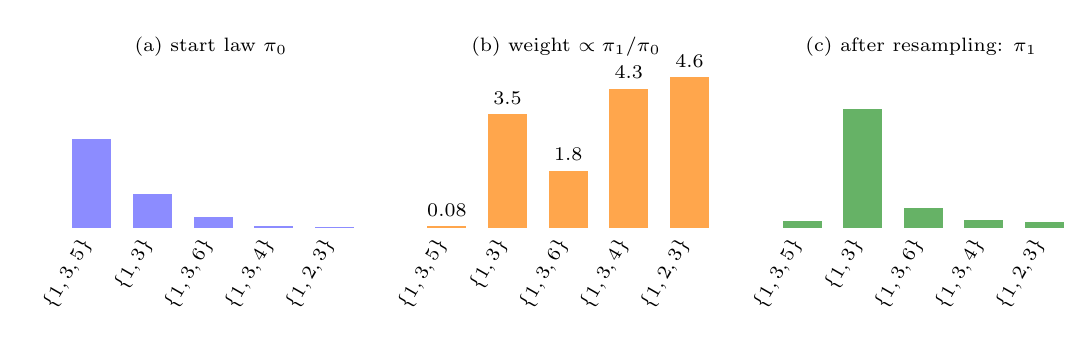
\begin{tikzpicture}[every node/.style={font=\scriptsize}, x=0.55cm, y=2.2cm]
\foreach \sx/\ttl in {0/{(a) start law $\pi_0$}, 8.2/{(b) weight $\propto\pi_1/\pi_0$}, 16.4/{(c) after resampling: $\pi_1$}}{
  \node at (\sx+3.2,1.05) {\ttl};
  \foreach \i/\m in {0/{\{1,3,5\}},1/{\{1,3\}},2/{\{1,3,6\}},3/{\{1,3,4\}},4/{\{1,2,3\}}}{
    \node[rotate=60, anchor=east] at (\sx+\i*1.4+0.45,-0.02) {$\m$};}}
\foreach \i/\v in {0/0.517,1/0.198,2/0.067,3/0.012,4/0.008}{\fill[blue!45] (\i*1.4,0) rectangle ++(0.9,\v);}
\foreach \i/\v/\lab in {0/0.081/0.08,1/3.47/3.5,2/1.76/1.8,3/4.25/4.3,4/4.6/4.6}{
  \fill[orange!70] (8.2+\i*1.4,0) rectangle ++(0.9,\v*0.19); \node[above] at (8.2+\i*1.4+0.45,\v*0.19) {\lab};}
\foreach \i/\v in {0/0.042,1/0.688,2/0.118,3/0.051,4/0.037}{\fill[green!50!black!60] (16.4+\i*1.4,0) rectangle ++(0.9,\v);}
\end{tikzpicture}
\caption{One reweighting step on the models of Example~\ref{ex:m-toy}, taken all the way from $\phi=0$ to $\phi=1$ with
very many particles. (a) Particles drawn from the start law sit mostly on $\{1,3,5\}$. (b) Each model's weight is
$e^{d(S)}$, proportional to $\pi_1/\pi_0$ (shown as the ratio of the two rows of the example's table): small for
$\{1,3,5\}$, large for $\{1,3\}$. (c) Resampling in proportion to these weights moves the mass to $\{1,3\}$, the highest
posterior model. The method takes many smaller steps instead, so that the weights stay even and the Markov
moves can spread the copies between steps.}
\label{fig:m-step}
\end{figure}

\subsection{The calibration (stage 4)}\label{sec:m-calibration}

The calibration answers two questions before the final run: which temperatures, and how many particles ($N_0$ or $4N_0$,
through the tier). It uses one short pilot island and a few rounds of four short diagnostic islands, and then
\emph{freezes} its answers before the final run draws any random number. At tier $i$ these islands have
$\Nc_i:=4^i\Nc_0$ particles, and the \emph{step ceiling} is $T_i:=4^i\max(1000,\ell_n^2)$.

\paragraph{Stores of models.} Throughout the run the method keeps three stores of the models scored so far: the $40p+1$
best by $F$; the $20p$ best by $\gamma_0$; and the $20p$ best by $\gamma_1=e^{F}/m(\emptyset)$, that is, by $F$. The two
stores of $20p$ feed the candidate set below. \emph{The best model found so far} is the model with the highest $F$ among
the models recorded so far: during the calibration, the block-table models (recorded before the pilot starts) and those
scored in the calibration; in the final run, the block-table models, those scored in the final run, and the models passed
on by the calibration.

\begin{center}
\fbox{\begin{minipage}{0.93\linewidth}\small
\textbf{Algorithm 1: calibration.}
\begin{enumerate}[leftmargin=1.6em,itemsep=1pt,label=\arabic*.]
  \item Set the tier $i\leftarrow0$.
  \item \emph{Pilot.} Run one island of $\Nc_i$ particles (reweight, resample, move, as in Section~\ref{sec:m-island})
    with an adaptive schedule. From the current $\phi$, the next temperature is $\phi'=1$ if that step keeps an effective
    sample size of at least $0.90\,\Nc_i$; otherwise it is found by 60 bisections on $(\phi,1]$. If the step is shorter than
    $1/T_i$, take $\phi'=\min(1,\phi+1/T_i)$ instead and count a \emph{forced step}. At $\phi=1$, run $L$ burn-in rounds and
    four measured rounds, then a local search (move cap $\ell_n$) from the best model found so far.
  \item \emph{Grid.} Build a grid from the pilot's temperatures on the candidate set $\mathcal V$ (below). If the
    construction fails, record a trigger and skip step~4.
  \item \emph{Rebuild loop.} Repeat at most $\ell_n$ times: run four diagnostic islands of $\Nc_i$ particles on the
    current grid (each as in Section~\ref{sec:m-island}, with $L$ burn-in and four measured rounds); run a local search
    (move cap $\ell_n$) from the best model found so far; recompute $\mathcal V$, and rebuild the grid from the pilot's
    temperatures. Stop when the rebuilt grid is identical to the previous one (the grid has \emph{converged}), or when a
    rebuild fails.
  \item \emph{Triggers.} If $i=0$ and any trigger fires (list below): repeat the check before the run, set $i\leftarrow1$,
    and go to step~2. The scored models, the three stores and the score cache carry over; the tier-$0$ temperatures do
    not, and tier~1 uses its own random streams. At tier~1, triggers are only recorded.
  \item \emph{Fallback.} If the grid construction failed at tier $1$, use the last grid built successfully at tier $1$,
    or else the tier-$1$ pilot's own temperatures. (An unconverged grid is used as it is.)
  \item \emph{Freeze} the grid, the tier $i$, the number of particles $N_i$ and $L$, and pass the three stores and the
    calibration's best model to the final run, as candidates for the reported model (they are not particles). With the
    fallback on (the default), a grid always exists at this point; if it does not, stop the run without estimates.
\end{enumerate}
\end{minipage}}
\end{center}

\paragraph{The candidate set and the grid.} The candidate set $\mathcal V$ is the empty model together with the two stores
of $20p$ models (the best by $\gamma_0$ and the best by $F$). On $\mathcal V$, let
$\psi(u):=\log\sum_{S\in\mathcal V}\gamma_0(S)e^{u\,d(S)}$. A step from temperature $u$ to $v$ has \emph{restricted effective
sample size}
\[
  \rho(u,v):=\exp\{2\psi(v)-\psi(u)-\psi(2v-u)\},
\]
the effective-sample-size fraction that the step would leave if the particles were the models of $\mathcal V$ with
weights proportional to $\gamma_u$. The grid \emph{refines} the pilot's temperatures. Starting at $u=0$, let $b$ be the
smallest pilot temperature above $u$. If $\rho(u,b)\ge0.90$, the next grid point is $b$; otherwise it is the largest
point of $(u,b]$ that passes, found by 60 bisections. The construction continues from the new point, again aiming at the
smallest pilot temperature above it, until it reaches $1$; so every pilot temperature is in the grid, and points are
inserted where a pilot step fails the check on $\mathcal V$. The construction \emph{fails} if a step
makes no numerical progress, if an appended temperature does not pass the $0.90$ check (temperatures within $10^{-12}$ of
$1$ are set to $1$), or if more than $T_i$ steps are needed.

\paragraph{Triggers.} At tier $0$ the calibration moves to tier $1$ if any of these occurs: \emph{island disagreement}
(E1: some diagnostic island's best log score is more than $1$ below the best score found so far); \emph{evidence
spread} (E2: the sample standard deviation of the four islands' log-evidence estimates exceeds $1$); \emph{late
improvement} (E3: a calibration local search, the pilot's included, ended with a strictly higher best log score than the
best before it started); a forced pilot step; a failed grid construction; a grid
that did not converge; or a local search that was still improving when it reached its move cap. E1 and E2 are taken from
the last completed rebuild; E3 and the move-cap trigger count over the pilot and every rebuild.

\paragraph{When the calibration succeeds.} The calibration \emph{succeeds} when it freezes a grid, built by the main
construction or by the fallback. Without a trigger, tier $0$ freezes its own grid. The calibration's own estimates are
archived and never reported.

\subsection{The final run and the local searches (stages 5 and 6)}\label{sec:m-search}

\paragraph{Final run.} Four independent islands of $N_i$ particles run on the frozen grid, each with its own, separately
seeded random-number stream (separate from the calibration's streams), starting from fresh draws from $\pi_0$.

\paragraph{Local search.} Two models are \emph{neighbours} if one comes from the other by deleting one predictor, adding
one (while the size is below $K$), or swapping one member for one non-member. A local search scans all neighbours of the
current model, scores each, and moves to the best one (ties broken lexicographically) if its log score is strictly
higher. It makes at most $c$ moves, where $c$ is its move cap. It stops at the first scan with no strict improvement,
and then certifies its end point (a local maximum of $F$). After the $c$-th move it still scans the neighbours once more:
if none improves, it certifies its end point; otherwise it returns the best improving neighbour as its end point,
uncertified, without moving there, and flags that it reached its cap. Every model scanned is recorded. After the islands, the
method runs two local searches:
\begin{itemize}[leftmargin=1.5em,itemsep=1pt]
  \item from the best model found so far (after the four islands), with move cap $\ell_n$;
  \item from the start mode $\tSz$, with move cap $\ell_n+\abs{\tSz}$. This search uses no random numbers and does not
    depend on the particles.
\end{itemize}

\subsection{What a run reports (stage 7)}\label{sec:m-outputs}

\paragraph{Output.} A run either \emph{produces output} (estimates), ending with status ``exact'' (enumeration) or
``completed'' (sampler), or it stops without estimates. A \emph{completed run} is a sampler run that delivered all the
estimates below.

\paragraph{The reported model and certification.} The method records every model it scores: all block-table subsets, the
models carried from the calibration, every particle and every proposal of the final islands, and every model scanned by
the two local searches. The \emph{reported model} $\Shat$ (the reported highest posterior model) is the best of them by
log score, with exact ties broken towards the smaller model and then lexicographically. The method \emph{certifies}
$\Shat$ (it sets its local-optimality flag) in two cases: (a) it enumerated $\Om$, so that $\Shat$ maximises $F$ over
$\Om$; or (b) $\Shat$ is the end point of a local search that stopped with no strict improvement, so that no neighbour of
$\Shat$ has a higher log score. In the exact case the method also sets a \emph{global-certificate} flag when $F(\Shat)$
exceeds every other score by more than a heuristic rounding-error margin; the flag is never set in the sampler case.

\paragraph{Exact case.} An exact run reports $\Shat$ (the highest posterior model), every inclusion probability
$\PIP_j$, the median probability model, $\log Z$, and both certificates.

\paragraph{Estimates.} The method pools the islands with equal weights:
\begin{equation}\label{eq:m-pool}
  \PIPhat_j:=\frac14\sum_{r=1}^4\PIPhat_{r,j},\qquad \Zhat:=\frac14\sum_{r=1}^4\Zhat_r,
\end{equation}
and reports $\Shat$, the pooled inclusion probabilities $\PIPhat_j$, the estimated median probability model
$\MPMhat:=\{j:\PIPhat_j>1/2\}$, $\log\Zhat$, the island estimates, and $\log(0.05\,\Zhat)$ as a one-sided 95\% lower bound
for $\log Z$. The bound rests on Markov's inequality, $\P(\Zhat>20Z)\le0.05$, which needs $\E\Zhat=Z$. The companion part
proves $\E(\Zhat\mid\text{calibration output})=Z$ for the estimate that the four islands would produce if the run were
not interrupted, on the event that the calibration succeeds, under its idealising conventions (exact arithmetic, ideal
random numbers, exact start sampler and kernels; Remark~5.22 and Convention (C3) there). This gives
$\P(\text{the run completes and }\Zhat>20Z)\le0.05$; it is not a 95\% coverage statement conditional on completion. Islands are not weighted by their evidence estimates.

\paragraph{Diagnostics.} The method reports, without changing any output: island disagreement (E1) and evidence spread
(E2) as in the calibration, computed on the final islands; late improvement (E3), whether the local search from the best
model strictly improved it (the search from the start mode is not counted); a low-effective-sample-size flag (some step
below $0.5N$); the models within $10^{-9}$ of the best log score among the store of the $40p+1$ best (with a flag when the store is full
and the list may be incomplete); whether either local search reached its move cap while
still improving; whether the search from the start mode improved the best model, or changed it without improving it (through the tie
rule); groups of correlated
predictors that span several blocks (components of the uncapped graph with edges $\abs{\hat r_{jl}}\ge\sqrt{2\log p/n}$,
not the neighbour graph); and the calibration's
own flags (move to tier~1, forced steps, unconverged grid, fallback).

\paragraph{Runs without estimates.} A run stops without estimates when its inputs are invalid; when no predictor or no
response variation remains; when the check before the run (memory and time), or its repeat before tier $1$, fails; when
the elapsed time plus the duration of the most recent operation would exceed the time allocation (checked after every
step, grid construction and local search); when all three score computations fail; or when no grid can be built.
Invalid inputs and a failed check before the run return no model; no retained predictor or a constant response returns
the empty model; any later stop returns the best model scored so far, marked incomplete. Every estimate is then marked
unavailable. Three cases end instead with an error and return nothing: an invalid allocation, and a violation of either
fixed integer limit of Table~\ref{tab:m-params} (the first is detected after the calibration, the second during the final
run).

% =====================================================================================================
\section{The parameter table}\label{sec:m-table}

Table~\ref{tab:m-params} lists the constants of the method. Each is a numerical constant or a function of $(n,p)$; the user sets only
the seed and the allocation, and the two switches marked ``on'' are the default configuration described here. The column
``Theory'' names the results of the companion part that use the constant (theorem numbers and conventions (C1)--(C3)
there); ``none'' means that no result depends on the value of the constant (the calibration constants, because the results
hold for every outcome of the calibration; the others, because they only affect reporting or computation). The example column uses $n=200$ and $p=10{,}000$. Code locations are relative to
\code{Scripts/SMC_BVS/core/}; code names, where they differ from the paper's symbols, are in parentheses.

{\footnotesize\setlength{\tabcolsep}{3.5pt}
\begin{longtable}{@{}>{\raggedright\arraybackslash}p{0.18\linewidth}>{\raggedright\arraybackslash}p{0.06\linewidth}>{\raggedright\arraybackslash}p{0.2\linewidth}>{\raggedright\arraybackslash}p{0.08\linewidth}>{\raggedright\arraybackslash}p{0.15\linewidth}>{\raggedright\arraybackslash}p{0.25\linewidth}@{}}
\caption{The constants of the method.}\label{tab:m-params}\\
\toprule
Parameter & Symbol & Value & {\scriptsize $n{=}200$, $p{=}10^4$} & Theory & Code \\ \endfirsthead
\toprule
Parameter & Symbol & Value & {\scriptsize $n{=}200$, $p{=}10^4$} & Theory & Code \\ \endhead
\grouprow{Prior}
size cap & $K$ & $\min(p,\lfloor n/2\rfloor)$ & 100 & all results & \code{cpp/v3_score.h:40}; \code{v3_preprocess.R:21} (\code{K}) \\
model prior $\BB(1,p)$ & $w(k)$, $\bar w_K$ & $\tfrac12/\binom{2p-1}{k}$, renormalised to $\Om$ & & all results & \code{cpp/v3_score.h:61-70} (\code{logw}, \code{logWK}) \\
coefficient prior scale; ridge & $g$ & $g=n$; unit ridge $I$ & 200 & all results & \code{cpp/v3_score.h:175-183} \\
inverse-gamma shape, scale & $a_0$, $b_0$ & $0.01$, $0.01$ & & all results & \code{cpp/v3_score.h:14} \\
\grouprow{Data preparation and score}
duplicate threshold & & $\abs{\hat r_{jl}}\ge1-10^{-10}$ (reported only) & & none & \code{cpp/v3_core.cpp:742-760} \\
small-$\SSq_S$ recomputation & & $\SSq_S<10^{-8}\,y^\top y$ & & none & \code{cpp/v3_score.h:219} \\
\grouprow{Blocks and start}
block size cap & $B$ & $\min(\lfloor\sqrt n\rfloor,\lfloor\sqrt p\rfloor,16)$ & 14 & Thms 5.2, 5.7, 5.12, 5.19 (the theorems use only $B\le16$: each predictor shares its block with at most 15 others) & \code{v3_preprocess.R:22}; cap 16 at \code{cpp/v3_core.cpp:145-146} (\code{B_MAX}) \\
neighbour threshold & & $\abs{\hat r_{jl}}>\sqrt{2\log p/n}$; 1 to $B$ neighbours before symmetrisation & 0.30 & none & \code{cpp/v3_blocks.h:146-172} \\
start-mode enumeration cap & & $10^6$, then tie-aware recursion & & (C2) & \code{cpp/v3_core.cpp:469}; \code{cpp/v3_start.h:271-305} \\
\grouprow{Exact case}
exact-case threshold & & enumerate if $\abs{\Om}\le(5\Nc_0+4N_0)p$ & $5.0\times10^8$ & scope of Cor 4.7, Thm 5.19 & \code{cpp/v3_core.cpp:71-85}; \code{v3_fit.R:105-106} \\
global certificate margin & & heuristic rounding bound, $64$ machine epsilons times a factor depending on the conditioning of $H_S$ & & none & \code{cpp/v3_score.h:240-246}; \code{cpp/v3_core.cpp:560-567} \\
\grouprow{Sampler}
islands & & $4$ & 4 & Thm 5.19, Rem 5.22 & \code{v3_run.R:91} (\code{islands}) \\
particles per island & $N_i$ & $4^i\max(2500,n,p)$ & 10,000 (tier 0), 40,000 (tier 1) & (C3) & \code{v3_preprocess.R:25,30} (\code{N0}) \\
burn-in rounds at $\phi=1$ & $L$ & $\max(4,\lceil\log_2(n+1)\rceil)$ & 8 & (C3) & \code{v3_preprocess.R:24} \\
measured rounds & & $4$ & 4 & (C3) & \code{v3_run.R:90}; \code{v3_calib.R:12} \\
resampling & & multinomial, every step & & (C3) & \code{cpp/v3_engine.h:230-259} (resampler), \code{:316-327} (use) \\
moves per round & & $p$ inclusion updates, 1 uniform swap, $B$ neighbour swaps, 1 independence move & 10,016 & (C3) & \code{cpp/v3_engine.h:111-214} \\
\grouprow{Calibration}
calibration particles & $\Nc_i$ & $4^i\lceil512N_0/2500\rceil$, $N_0:=\max(2500,n,p)$ & 2,048; 8,192 & none & \code{v3_preprocess.R:26,30} (\code{H0}) \\
step ceiling & $T_i$ & $4^i\max(1000,\ell_n^2)$ & 1,000; 4,000 & none & \code{v3_preprocess.R:27,30} (\code{T0}) \\
tiers & $i$ & $i\in\{0,1\}$, factor $4^i$, at most one move to tier 1 & & none & \code{v3_preprocess.R:30}; \code{v3_calib.R:150-159} \\
pilot effective-sample-size target & & $0.90\,\Nc_i$ & 1,843.2 (tier 0) & none & \code{cpp/v3_calib.h:31} \\
pilot step floor & & $1/T_i$ & 0.001 (tier 0) & none & \code{cpp/v3_calib.h:38-43} \\
grid target & & $\rho\ge0.90$ & & none & \code{cpp/v3_calib.h:79,84,92} \\
bisections & & 60 & & none & \code{cpp/v3_calib.h:34,82} \\
candidate set & $\mathcal V$ & $\emptyset$, best $20p$ by $\gamma_0$, best $20p$ by $F$ & up to 400,001 & none & \code{cpp/v3_core.cpp:699-724}; \code{cpp/v3_ledger.h:78} \\
rebuild iterations & & at most $\ell_n$ & 14 & none & \code{v3_calib.R:84-119} \\
triggers E1, E2 & & gap $1$ in log score; s.d.\ $1$ of $\log\Zhat_r$ & & none & \code{v3_calib.R:101-102} \\
diagnostic islands per rebuild & & $4$ & 4 & none & \code{cpp/v3_core.cpp:664} \\
snap to $\phi=1$ & & within $10^{-12}$ & & none & \code{cpp/v3_calib.h:42,89} \\
grid fallback & & on & & Thms 5.7, 5.12 (delivery) & \code{v3_calib.R:120-125,163-169}; \code{v3_fit.R:151} \\
\grouprow{Local searches}
base move cap & $\ell_n$ & $\lceil\log_2(n+p+1)\rceil$ & 14 & Thms 5.7, 5.12 & \code{v3_preprocess.R:23} (\code{ell}) \\
move cap from the start mode & & $\ell_n+\abs{\tSz}$ & & Thms 5.7, 5.12 & \code{cpp/v3_core.cpp:473}; \code{v3_run.R:100-101} (\code{ls0_cap}) \\
search from the start mode & & on & & (C1); Thms 5.7, 5.12 & \code{v3_fit.R:73} (\code{ls0 = TRUE}); \code{cpp/v3_core.cpp:460-481} \\
\grouprow{Outputs}
pooling of islands & & equal weights & & Thm 5.19, Rem 5.22 & \code{v3_run.R:154,162} \\
estimated MPM threshold & & $\PIPhat_j>1/2$ & & Thm 5.19 & \code{v3_run.R:163} \\
stored models & & best $40p+1$ by $F$ & 400,001 & Cor 4.7 & \code{cpp/v3_ledger.h:78} \\
evidence lower bound & & $0.05\,\Zhat$ & & none & \code{v3_run.R:155} \\
low-effective-sample-size flag & & below $0.5N$ at some step & 5,000 (tier 0) & none & \code{v3_run.R:201} \\
near-tie window & & $10^{-9}$ in log score & & none & \code{v3_run.R:171} \\
\grouprow{Computing}
allocation defaults & & 8\,GiB ($8\cdot2^{30}$ bytes), 24\,h & & (C2) & \code{v3_fit.R:28,47,60,73,92} \\
score cache & & $500p$ models, cleared when full & $5\times10^6$ & none & \code{v3_run.R:92}; \code{v3_calib.R:147} \\
check before the run & & memory; exact case: time of 200 timed scores $\times$ count; sampler: worst-case time $2(\ell_n+K+1)(p+p^2/4)\times$(time of a size-$K$ score) & $2.9\times10^9$ requests & (C2) & \code{v3_fit.R:10-14,26-68,114-117,144-148} \\
random streams & & 0--4 (tier 0), 5--9 (tier 1), 10--13 (final islands) & & (C3) & \code{v3_run.R:8-11}; \code{cpp/v3_core.cpp:444,626,667} \\
seed & & integer in $[1,2^{31}-1]$ & & (C1) & \code{v3_preprocess.R:7-11} \\
\grouprow{Two fixed integer limits (facts of the code)}
ceiling on the base move cap & & $\ell_n\le10^6$, else the run ends with an error & & delivery domain $\Dom$ & \code{v3_run.R:96} \\
integer range of the move cap & & $\ell_n+\abs{\tSz}\le2^{31}-1$, else the run ends with an error & & delivery domain $\Dom$ & \code{cpp/v3_core.cpp:474} \\
\bottomrule
\end{longtable}}

The two limits at the end of the table are facts of the code, not tuning choices. The first can bind only when $n+p+1$
exceeds $2^{10^6}$; the second only when the start mode has more than about $2.1\times10^9$ predictors, which needs
$n\gtrsim4.3\times10^9$, since $\abs{\tSz}\le\lfloor n/2\rfloor$.

\bibliography{../shared/refs}

\appendix
% =====================================================================================================
\section{The engine for $p=10^6$ (an engineered variant)}\label{app:m-1m}

\emph{This appendix describes a different engine, not the method above. The theorems of the companion part are about the
method above.} To run at $p=10^6$, the planned engine changes the method as listed in Table~\ref{tab:m-1m}, taken from the
draft engineering specification of 2026-11-15; entries marked ``to be decided'' depend on a precision study. The run at
$p=10^6$ will be reported as an engineered variant validated against the method above on shared problem sizes ($p=10^4$,
and $p=10^5$ where possible), not as a run covered by the theorems.

{\small
\begin{longtable}{@{}>{\raggedright\arraybackslash}p{0.2\linewidth}>{\raggedright\arraybackslash}p{0.33\linewidth}>{\raggedright\arraybackslash}p{0.4\linewidth}@{}}
\caption{The $10^6$ engine against the method.}\label{tab:m-1m}\\
\toprule
Aspect & The method & The $10^6$ engine \\ \midrule \endhead
particles per island & $4^i\max(2500,n,p)$ & fixed, $2{,}500$ ($10^4$ in one arm of the precision study) \\
islands & four, in one process & sixteen, in separate processes, merged afterwards (union of stored models; equal-weight inclusion probabilities as the primary estimate) \\
random numbers & sequential streams & addressed by position (counter-based) \\
scoring & the score of Section~\ref{sec:m-posterior} & a batched kernel with different floating-point arithmetic, agreeing to about $10^{-9}$ in relative terms \\
blocks & the partition of Section~\ref{sec:m-blocks}, $B\le16$ & complete linkage truncated at a correlation threshold, the same top-down cut, packing by smallest index; $B\le14$ \\
calibration & Algorithm~1, with at most one move to tier 1 & the pilot and at most a fixed number of rebuilds (0 or 3, to be decided), no move to tier 1 except after a failed construction \\
grid & as frozen & optionally each interval split into $m\in\{1,4\}$ equal parts (to be decided) \\
estimates & those of Section~\ref{sec:m-outputs} & the same, plus a deterministic lower bound on $\log Z$ from the stored models, an evidence estimate based on how often the islands visit the stored models, and inclusion probabilities computed from the stored models \\
resampling and moves & multinomial; $B$ neighbour swaps per round & systematic resampling and more neighbour swaps per round, off unless the precision study shows a gain \\
caches & a score cache, the store of the $40p+1$ best models, and the two stores of $20p$ & no score cache and no stores of $20p$ in the final islands; each island keeps a store of its $40p+1$ best models \\
\bottomrule
\end{longtable}}

% =====================================================================================================
\section{Notation specific to this part}\label{app:m-notation}

The symbols of Sections~\ref{sec:m-setup}--\ref{sec:m-posterior} are shared with the companion part, whose notation
table lists them. The symbols specific to this part are:

{\small
\begin{longtable}{@{}p{0.22\linewidth}p{0.58\linewidth}l@{}}
\toprule
Symbol & Meaning & Where \\ \midrule \endhead
$B$ & block size cap $\min(\lfloor\sqrt n\rfloor,\lfloor\sqrt p\rfloor,16)$ & \S\ref{sec:m-blocks} \\
$\hat r_{jl}$ & sample correlation of predictors $j$ and $l$ & \S\ref{sec:m-data} \\
$N_0$, $\Nc_0$ & $\max(2500,n,p)$; $\lceil512N_0/2500\rceil$ & \S\ref{sec:m-budgets} \\
$\mathcal N(j)$ & neighbours of predictor $j$ & \S\ref{sec:m-blocks} \\
$C_b$, $J$, $r_b(U)$ & blocks; number of blocks; block table $m(U)/m(\emptyset)$ & \S\ref{sec:m-blocks} \\
$\gamma_0$, $\bar Z_0$, $\pi_0$ & unnormalised start law; its normaliser; start law & \S\ref{sec:m-start} \\
$E_b(k)$, $\Phi_b(k)$ & table weight of block $b$ at size $k$; cumulative size profile & \S\ref{sec:m-start} \\
$\tSz$ & start mode & \S\ref{sec:m-start} \\
$d(S)$ & discrepancy between the posterior and the start law & \S\ref{sec:m-start} \\
$\phi$, $\gamma_\phi$, $\pi_\phi$; $\grid t$, $T$ & temperature; path from the start law to the posterior; grid; number of stages & \S\ref{sec:m-island} \\
$N_i$, $L$, $\omega^{(t)}_s$, $o_j$, $a$ & particles per island at tier $i$; burn-in rounds; reweighting factor; conditional inclusion probability (Gibbs); its odds & \S\ref{sec:m-island} \\
$r$; $\PIPhat_{r,j}$, $\Zhat_r$ & island index; island estimates & \S\ref{sec:m-island} \\
$i$; $\Nc_i$, $T_i$; $\ell_n$ & tier; calibration particles and step ceiling; base move cap & \S\ref{sec:m-calibration} \\
$\mathcal V$, $\psi$, $\rho$ & candidate set; restricted log-normaliser; restricted effective-sample-size fraction & \S\ref{sec:m-calibration} \\
E1, E2, E3 & island disagreement; evidence spread; late improvement & \S\ref{sec:m-calibration} \\
$\Shat$, $\PIPhat_j$, $\Zhat$, $\MPMhat$ & reported model and pooled estimates & \S\ref{sec:m-outputs} \\
\bottomrule
\end{longtable}}

% =====================================================================================================
\section{Where the sources and the code disagree (internal; removed for submission)}\label{app:m-disagree}
Checked against the code by an independent reader (2026-11-16). In each case this text follows the code.
\begin{enumerate}[leftmargin=1.8em]
  \item The earlier method chapter (\code{Theory_work/State_of_Project/sections/02_method.tex:440-451}) describes an
    evidence-weighted pooled inclusion probability as primary, and \code{Docs/Methodology/METHODOLOGY_v3.md:272-274} as
    secondary; the code pools the islands with equal weights and computes neither (\code{v3_run.R:154,162};
    \code{README.md:16}). This text follows the code.
  \item A code comment says the block size satisfies $1\le B\le20$ (\code{cpp/v3_core.cpp:144}); the constant is $16$
    (\code{cpp/v3_core.cpp:145-146}). This text uses $16$.
  \item The earlier method chapter (\code{Theory_work/State_of_Project/sections/02_method.tex:363-400}) describes an optional
    number of final islands $R'=4k$, declared in advance, with an ``expanded'' and a ``baseline'' record, and a parallel
    execution layer with process workers. The shipped serial code fixes the number of islands at four
    (\code{v3_run.R:91}, \code{islands = 4L}) and has neither option. This text describes four islands; the parallel
    engine is the subject of Appendix~\ref{app:m-1m} and of Section~6 of the companion part.
  \item \emph{The check before the run.} \code{README.md:19} and the code comment at \code{v3_fit.R:25} say the
    sampler's check is memory-only; \code{METHODOLOGY_v3.md:321-324,403} describes a memory and time check for both
    branches. In the default configuration the code checks memory and the worst-case time of the search from the start
    mode (\code{v3_fit.R:114-117, 43-47}), before the run and before tier~1 (\code{:144-148}). \code{02_method.tex:507}
    quotes an overhead of that search ``under 1\,s per fit''. This text follows the code (Section~\ref{sec:m-budgets}).
  \item The move cap of the search from the start mode is $\ell_n+\abs{\tSz}$ in the code (\code{cpp/v3_core.cpp:473-479};
    \code{v3_run.R:100-101}); \code{02_method.tex:492} and \code{README.md:43} give $\ell_n$.
  \item The fallback for a failed tier-1 grid is on by default (\code{v3_calib.R:120-125,163-170}; \code{v3_fit.R:151});
    \code{METHODOLOGY_v3.md:226} and \code{02_method.tex:324-325} say such a run stops (\code{schedule_limit}).
  \item \code{METHODOLOGY_v3.md:57,158} calls the exact case's global certificate validated; the code labels its bound
    heuristic (\code{cpp/v3_score.h:240-246}).
  \item Items of \code{02_method.tex} not in the code: a near-tie window $\max(10^{-9},2\eta)$ (\code{:485}; the code uses
    $10^{-9}$, \code{v3_run.R:171-173}); plain inclusion probabilities (\code{:452-456}); the statuses
    \code{degenerate_n} and \code{unsupported_size} and $n=2$ (\code{:59-62}; the code rejects $n<3$,
    \code{v3_preprocess.R:106}); a certificate card and related bounds (\code{:427-431, 512-576}).
  \item The line numbers cited in \code{02_method.tex} refer to a campaign copy of the code, not to
    \code{Scripts/SMC_BVS/core/}, and do not transfer.
  \item \code{METHODOLOGY_v3.md:38} gives the default memory allocation (8\,GiB, as in the code) but not the default time
    allocation of 24 hours (\code{v3_fit.R:73,92}). \code{METHODOLOGY_v3.md} \S6.1 and \S6.10 do not describe the search from the start mode or
    the tie-aware start-mode recursion, both on by default in the code.
\end{enumerate}

\end{document}
